\section{Double Ratchet Algorithm}
\label{ch:dr}

The Double Ratchet is a cryptographic asynchronous message exchange algorithm that provides high security to the communicating parties. The algorithm enables the exchange of encrypted messages based on a shared secret key between the two parties where each message is encrypted with its specific ephemeral key.
The double ratchet algorithm is a combination of two ratchet constructions which provide enhanced security properties.
The first outer ratchet is inherited from \gls{otr}'s asymmetric ratchet to benefit from its future secrecy property which is obtained through the use of ephemeral key exchanges. Coupled by an inner symmetric ratchet for forward secrecy, the algorithm was formed and was formerly named Axolotl Ratchet. Additionally, \gls{kdf} chains are a core concept of the algorithm. This section goes through the methodology of the algorithm, its features, and its security properties.

\subsection{\gls*{kdf} Chain}
As mentioned in section \ref{backgroung:kdf}, a \gls{kdf} is a function that takes as input a key and an input and produces a cryptographically secure hash output that is random-like.
A \gls{kdf} chain is a series of connected \gls{kdf}s where one output key of a \gls{kdf} is a \gls{kdf} key input of a succeeding \gls{kdf}. Figure \ref{fig:kdf-chain} shows an illustration for a \gls{kdf} chain that takes three external inputs and produces three random output keys.

\begin{figure}[hptb]
	\centering
	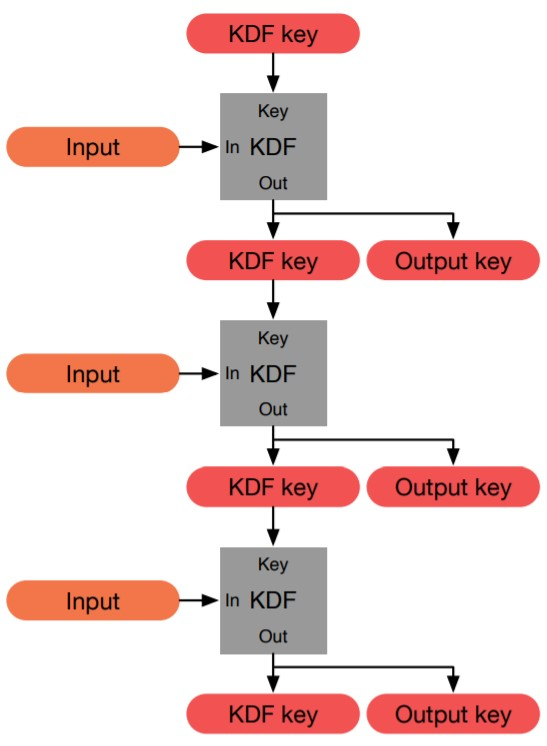
\includegraphics[scale=0.4]{Images/kdf-chain.jpg}
	\caption{A 3 input KDF chain \cite{dblRtcht}.}
	\label{fig:kdf-chain}
\end{figure}

The algorithm session has three \gls{kdf} chains: Root chain, sending chain, and receiving chain. Each chain is advanced whenever its relevant ratchet performs a step. More details about ratchet steps and their relation to the \gls{kdf} chains are discussed in later sections.
\par
KDF chains have a set of characteristics:
\begin{itemize}
	\item \textit{Resilience:} An adversary who does not know the KDF keys perceives the output keys as random. Even if the opponent has complete control over the KDF inputs, this is still valid.
	
	\item \textit{Forward secrecy:} An adversary who discovers the KDF key at some point in the future cannot distinguish between past output keys and random.
	
	\item \textit{Future secrecy:} If future inputs have contributed adequate randomness, future output keys seem random to an adversary who learns the KDF key at some point in the future.
\end{itemize}

\subsection{Symmetric-key Ratchet}
	
The sending and receiving chains are constructed of symmetric-key ratchets where Alice's sending chain is equivalent to Bob's receiving chain and vise versa. Essentially, a symmetric-key ratchet is a \gls{kdf} chain with a constant input through out the chain steps. However, unlike with random input, a constant input does not provide future secrecy.
\par
In a symmetric-key ratchet, the KDF key illustrated in figure \ref{fig:kdf-chain} is the chain key, while a KDF's output key is a unique message key. For a sending chain, a message key is used to encrypt the outgoing message. On the other side, a message key in the receiving chain is used to decrypt the incoming message. The process of calculating the next chain and message keys is an advance in the sending/receiving chain. This is referred to as a \textit{symmetric ratchet step}.
\par
Message keys are not re-introduced into the KDF chain, therefore, they can be discarded without proposing any security risk to earlier or later ratchet outputs. Also, it is possible to store message keys to handle out-of-order messages on the receiving end. Storing message keys introduce a risk to only their respective messages. However, a compromise of a chain key can lead to further compromise of future chain keys as future chain keys rely on previous ones.

\subsection{Diffie-Hellman Ratchet}
The \gls{dh} ratchet provides the future secrecy property. When paired with the symmetric ratchet, the combination addresses the symmetric ratchet lack of future secrecy. 
Each party generates a \gls{dh} key pair known as their \textit{ratchet key pair}. The parties exchange their public keys within message headers with which each can compute an equivalent \gls{dh} secret output using their own private key that is equivalent to the public key they sent. The process of generating a new \gls{dh} output when receiving a new public key is referred to as a \textit{\gls{dh} ratchet step}. Accordingly, a passive adversary that compromises one party's private key at a point in time is incapable of deducing the upcoming \gls{dh} outputs due to the use of newly generated key pair for each ratchet step.
\par
Next, we discuss an algorithm run where a \gls{dh} ratchet is advanced to create two different DH secret outputs between Alice and Bob. Bob is assumed to be the algorithm initiator. Figure \ref{fig:dh-bobRatchet} serves as visual aid for our discussion where we proceed in steps as labeled in the diagram.

\begin{figure}[hptb]
	\centering
	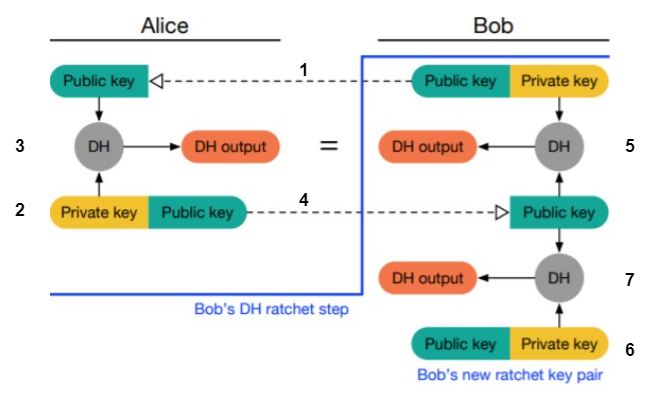
\includegraphics[scale=0.6]{Images/dr-bobRatchet.png}
	\caption{Bob \gls{dh} Ratchet step. Figure reproduced from \cite{dblRtcht}.}
	\label{fig:dh-bobRatchet}
\end{figure}

\begin{itemize}
	\item \textit{Step 1:} Bob generates his first ratchet key pair to send the initial message to Alice. The initial message header contains Bob's public key. 
	
	\item \textit{Step 2:} Upon receiving Bob's public key, Alice generates her ratchet key pair.
	
	\item \textit{Step 3:} Alice performs a \gls{dh} calculation between her private key and Bob's public key generating her side of the DH output.
	
	\item \textit{Step 4:} Alice advertises to Bob her public portion of her ratchet key pair that was used to generate the DH output.
	
	\item \textit{Step 5:} After obtaining Alice's ratchet public key, Bob performs a DH calculation between it and his current ratchet private key resulting in Bob's copy of the shared DH output.
	
	\item \textit{Step 6:} Furthermore, Bob generates a new ratchet key pair to generate the next DH output.
	
	\item \textit{Step 7:} Bob performs a \gls{dh} calculation between hit new ratchet private key and Alice's public key generating a new DH output.
\end{itemize}
The steps described above are Bob's DH ratchet step as Bob was the initiator of the ratchet step by advertising his public key. Similarly, Alice's ratchet step starts by sending her public key to Bob and concludes after performing the same steps mentioned above but with the roles reversed.
\par
Linking the algorithm to the messaging context, the DH outputs represent the sending and receiving chains' root keys. The party advancing its ratchet, say Bob, results in Alice generating the sending chain root key and Bob generating the receiving chain root key, and vice versa.
\par
However, the description so far is simplified. The algorithm is augmented by a KDF chain to improve resilience and future secrecy. The KDF chain key is a shared secret between both parties while the KDF inputs are the DH outputs from the DH ratchet. Every step through the KDF chain results in a new kdf root key and a sending/receiving chain root key. So a full DH ratchet step consists of updating the root KDF chain twice generating both a sending and a receiving chain key. Figure \ref{fig:dh-ratchet_chain} illustrates a full DH ratchet step.

\begin{figure}[hptb]
	\centering
	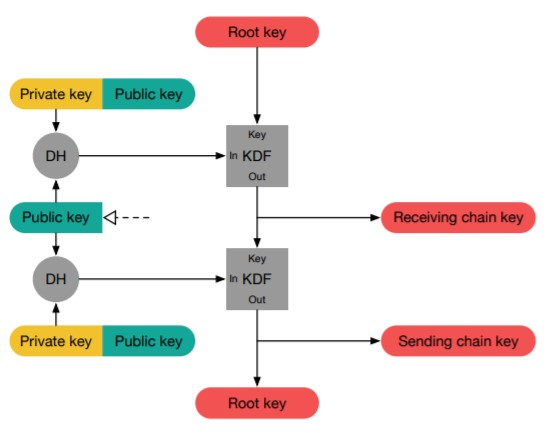
\includegraphics[scale=0.6]{Images/fullDHRatchetStep.jpg}
	\caption{A full \gls{dh} Ratchet step \cite{dblRtcht}.}
	\label{fig:dh-ratchet_chain}
\end{figure}

\subsection{Double Ratchet}

\subsection{Out-of-order Messages}

\subsection{Header Encryption}

\subsection{Integration with \gls*{x3dh}}

\subsection{Formal Verification}

\subsection{Post-Quantum Security}
